\documentclass{article}
\usepackage{xcolor} % for different colour comments
\usepackage{graphicx}
\graphicspath{{images/}}
\usepackage{tabu}
\usepackage{float}

%% Comments
\newif\ifcomments\commentstrue
\newcommand{\cs}[1]{\authornote{blue}{cs}{#1}} %Connor
\newcommand{\dm}[1]{\authornote{blue}{dm}{#1}} %Danny
\newcommand{\sm}[1]{\authornote{blue}{SM}{#1}} %Shani
\renewcommand*\contentsname{Table of Contents}
\begin{document}
%Text in red represents major changes made to the document after Revision 0.
\title{OpenBazaar Redevelopment - Requirements}
\author{The Fair Traders \\ Daniel Mandel - mandeldr \\ Shandelle Murray - murras25 \\ Connor Sheehan - sheehacg}
\date{\today}
\maketitle
\begin{abstract}
This documents outlines requirements for the OpenBazaar redevelopment project.
\end{abstract}
\newpage
\tableofcontents
\newpage
\addcontentsline{toc}{section}{Revision History}
\section*{Revision History}


\begin{table}[H]
\centering
\begin{tabu} to 1\textwidth {|| X[l] | X[l] | X[l] | X[l] ||}
 \hline
 Revision Number & Revision Date & Description of Change & Author \\ [0.5ex] 
 \hline\hline
 1 & November 2nd, 2015 & Created Revision History & Daniel Mandel \\ [1ex] 
 \hline
 2 & November 10 - November 20, 2015 & Add non-functional requirements  & All members of group \\ [1ex]
 \hline
 3 & November 25, 2015 & Section 4.1 - Kademlia and Ricardian Contract defined  & Shandelle Murray \\ [1ex]
 \hline
 4 & November 28, 2015 & Sections 6.2 and 6.3 - Add context diagram and work partitioning table, create lists of figures and tables  & Shandelle Murray \\ [1ex]
 \hline
 5 & December 8, 2015 & Add use case diagram, remaining non-functional requirements, and last sections  & Shandelle Murray \\ [1ex]
 \hline
 
\end{tabu}
\caption{Table to capture the history of the document}
\label{table:1}
\end{table}
\addcontentsline{toc}{section}{References}
\section*{References}
We have used the Volere Template as a guide for creating this requirements document.\newline
\newline
http://docs.openbazaar.org/ was also referenced for material regarding the OpenBazaar.
\addcontentsline{toc}{section}{Project Drivers}
\section*{Project Drivers}
\section{The Purpose of the Project}
\subsection{The User Business or Background of the Project Effort}
The modern economic era is built around e-commerce and internet trade. This is apparent from the change in the speed of stock market trades, the explosion of technology based corporations and the expansion of internet commerce services such as Alibaba and eBay.
Currently, people who wish to buy and sell online are largely constrained to utilizing the services offered by the large corporations, thereby sacrificing a portion of the profit from trades. In undertaking the OpenBazaar project, we aim to benefit both online buyers and sellers by creating a platform in which internet trade can be decentralized
The project will be developed as an open-source, peer-to-peer network. 
\subsection{Goals of the Project}
The main goals of the project include:
\begin{itemize}
\item
Creating an online marketplace that is scalable, free of intermediaries and their fees, and cannot be censored.
\item
Eliminating the need for centralized e-commerce services and websites.
\item
Reducing the overhead cost of doing business and trading over the internet by using the software which will essentially make trade free again.
\item
Creating a permission-less, censorship-resistant trade platform that will connect the entire world.
\end{itemize}
\section{The Stakeholders}
\subsection{Traders}
At the present time, anyone who wishes to open an online store must use a centralized service. These services often charge listing fees, subscription fees or membership fees. Traders are also forced to use centralized exchange platforms such as PayPal or be charged bank fees for direct deposits. Traders stand to benefit from the project by the elimination of both of these unnecessary expenditures. The use of BitCoin will allow for a fee-less monetary exchange and a free product listing on the OpenBazaar network.
\subsection{Buyers}
Buyers who shop online will benefit from this project in several ways. The overhead costs of doing trade will be lower on this platform than centralized services, and buyers should expect to see a reflection of this in the prices of products on OpenBazaar. Buyers will be free to exchange goods with anyone they can connect to on the network, 
\subsection{Other Stakeholders}
Other stakeholders include:
\begin{itemize}
\item
Major corporations that currently benefit from trades between buyers and sellers through the internet
\item
Collectively, law enforcement can be considered a stakeholder as they will be affected by this new form of online trade and will likely have to alter their tactics for detecting illegal online activity
\item
Members of the development team
\item
Computer/internet users in general may be considered stakeholders because, with a simpler and more effective manner of completing sales and trades readily available, more of these people may turn to internet trading
\end{itemize}
\subsection{The Hands-On Users of the Product}
The hands-on users of the product:
\begin{itemize}
\item
Online Sellers/Traders
\item
Online Buyers
\item
Computer/internet users interested in buying and selling online
\end{itemize}
\subsection{Priorities Assigned to Users}
\begin{itemize}
\item
Key Users: Online buyers and sellers
\item
Secondary Users: Developers and testers
\end{itemize}
\subsection{User Participation}
\begin{itemize}
\item 
Users acting as prospective buyers, sellers, or an anonymous, third-party mediator access the OpenBazaar network                
\item
Users acting as sellers advertise their products on the OpenBazaar network
\item
Users acting as buyers browse or search for products that they would like to buy on the OpenBazaar network
\item
Users acting as notaries advertise their mediation services on the OpenBazaar network and serve as a third party to ensure a fair trade
\end{itemize}
\subsection{Maintenance Users and Service Technicians}
\begin{itemize}
\item
Developers and Testers
\end{itemize}
\addcontentsline{toc}{section}{Project Constraints}
\section*{Project Constraints}
\section{Mandated Constraints}
\subsection{Solution Constraints}
\begin{itemize}
\item
Description: The OpenBazaar client will run on Windows, Linux and Mac OS X. 
\item
Rationale: These are three of the most common desktop software platforms available. 
\item
Fit Criterion: The required framework and programming language must be installed (PyQT 4, Python 2).
\item
Description: In order to have full functionality a working internet connection is necessary.
\item
Rationale: The internet is the fastest way to connect buyers and sellers around the globe and exists in most modernized countries.
\item
Fit Criterion: It is required to make transactions, view markets, and discover peers on the network.
\item
Description: To make trade completely decentralized, as well as entice buyers and sellers to connect over the OpenBazaar marketplace, Bitcoin must be used as a currency. 
\item
Rationale: It is the easiest as well as one of the safest ways to make transactions over the internet. it is also becoming more and more accepted in other retail and online stores. 
\item
Fit Criterion: Users must have a Bitcoin wallet installed on their computer. 
\end{itemize}
\subsection{Implementation Environment of the Current System}
\begin{itemize}
\item
The application will be developed on Ubuntu 14, using Python 2, and PyQT as the GUI framework. The framework was chosen because of its cross-platform abilities and versatility. Ubuntu was chosen because of the compatibility it has with the existing off-the-shelf software’s (OpenBazaar Server), Git, and the other partner applications that make OpenBazaar function. 
\end{itemize}
\subsection{Partner or Collaborative Applications}
\begin{itemize}
\item
BitCoin will be a vital application serving as the medium of exchange on OpenBazaar.
\end{itemize}
\subsection{Off-the-Shelf Software}
\begin{itemize}
        
\item
There is an existing off-the-shelf software, but it is in the beta development phase, with development focus on the front end (back-end complete) and testing. The front end or client side of the application will act similarly to an online classifieds system like Ebay, Amazon, Kijiji, Craigslist; however, it will be populated with only what a user would like to see. 
        
\end{itemize}
\subsection{Anticipated Workplace Environment}
\begin{itemize}
        
\item
This system is intended for use anywhere that there is a working internet connection. This enables users to connect from all around the world to buy and sell products and services. Virtually, the anticipated workplace environment is the entire civilized world.
        
        
\end{itemize}
\subsection{Schedule Constraints}
\begin{itemize}
        
\item
This project should be completed and tested by November 30, 2015
\item
Learning should be focused on the PyQt4 framework, and creating wireframes for the GUI.
\item
Final documentation must be complete by December 8, 2015.
        
\end{itemize}
\section{Naming Conventions and Terminology}
\subsection{Definitions of All Terms}
\begin{itemize}
        
\item
Python: a widely used and versatile high level programming language
\item
IDE: integrated development environment
\item
PyCharm: the chosen IDE for the project 
\item
GUI: Graphical User Interface
\item
Git: source control for the project, includes features such as revision history
\item
Bitcoin: digital store of value and online payment system
\item
Ricardian contract: used for the purpose of issuing digital currency, it is a document which states the terms under which a value is redeemable. It is readable by people, parsable by programs, and prevents unauthorized changes by making use of digitally signed and checksum hashed contracts. The contract carries keys and server information, and requires digital signatures of the issuer, a holder, and possibly a third-party notary in order for a value to be redeemed.
\item
Kademlia DHT: a distributed hash table for decentralized peer-to-peer computer networks that is designed to minimize the number of configuration messages nodes must send to learn to about other nodes.
\end{itemize}
\section{Relevant Facts and Assumptions}
\subsection{Assumptions}
\begin{itemize}
        
\item
It is assumed that any user of the application understands the Bitcoin currency.
\item
It is assumed that end users understand how a peer-to-peer application is different from the traditional client-server model.
\end{itemize}
\subsection{Facts}
\begin{itemize}
        
\item
There are existing frameworks for GUIs. PyQt in particular will be used for the implementation of the client side. 
\item
We will be focusing on developing the client side of the application due to the time constraint of this project.
        
\end{itemize} 
\section{The Scope of the Work}
\subsection{The Current Situation}
\subparagraph{Content}
A software application to connect users from all around the world to conduct trade freely is required. Users can add any peers to the network, as well as view their stores, and search for items to purchase. They will also have the ability to have their own store to sell items.
\subsection{The Context of the Work}
\begin{figure}[H]
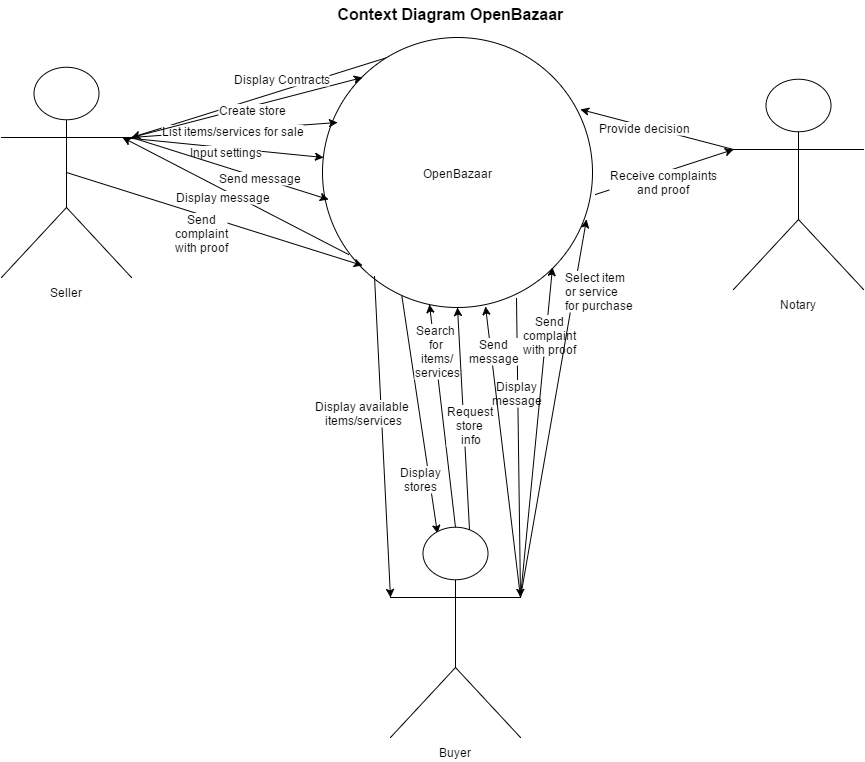
\includegraphics[scale=0.5]{ContextDiagramOpenBazaar}
\caption{\textcolor{red}{Context Diagram OpenBazaar}}
\end{figure}

\subsection{Work Partitioning}
\begin{table}[H]
\color{red}
\centering
\begin{tabu} to 0.8\textwidth {|| X[l] | X[l] | X[l] ||}
 \hline
 \textbf {Event Name} & \textbf{Input and Output} & \textbf{Summary} \\
 \hline
 1.User inputs store information & Store Information (IN) & Seller saves store information \\
 \hline
 2.User inputs new contract information & Contract (IN), Contract (OUT) & Seller lists new item for sale and it is listed in their store \\
 \hline
 3.User inputs settings & Settings (IN) & User specifies personal or store settings \\
 \hline
 4.User sends complaint with proof & Complaint (IN), Complaint (OUT) & Buyer or seller generates complaint and notary receives it \\
 \hline
 5.User sends messsage & Message (OUT), Message (IN) & User sends message and another user receives message \\
 \hline
 6.User searches for listings & Search Criteria (IN), Available Listings (OUT) & User searches for avaiable listings and application displays them \\
 \hline
 7.User searches for store & Store ID (IN), Store (OUT) & User searches for store and application displays store \\
 \hline
 8.User requests to purchase listing & Purchase Request (IN), Updated Contract (OUT) & User requests to purchase item or service and application advances contract to next step \\
 \hline
 9.User provides decision about complaint & Decision (IN), Decision (OUT) & Notary makes ruling in favor of eithe party and application proceeds to complete the transaction according to the contract \\
 \hline
\end{tabu}
\caption{Table to capture the inputs and outputs of an event}
\label{table:2}
\end{table}

\section{The Scope of the Product}
\subsection{Product Use Case}
\begin{figure}[H]
	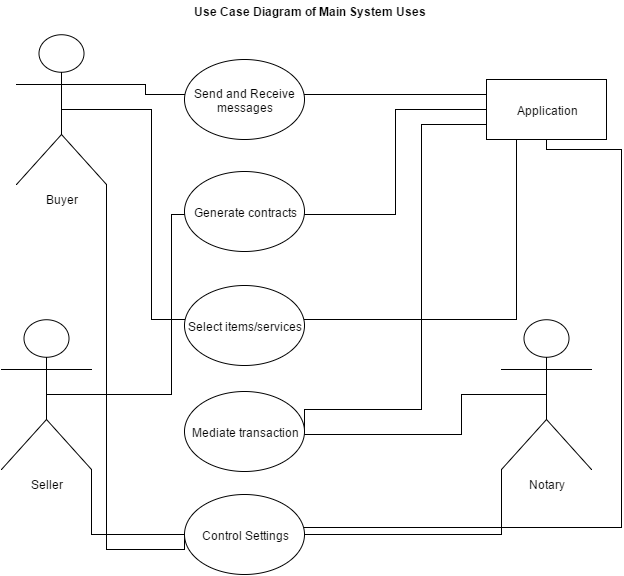
\includegraphics[scale=0.5]{usecase}
	\caption{\textcolor{red}{Use Case Diagram}}
\end{figure}


\addcontentsline{toc}{section}{Functional Requirements}
\section*{Functional Requirements}
\begin{description}
	%Requirements were changed due to the networking part of the application not being feasible to implement in the given timeframe. The original requirements are shown as comments.
%\item[R1]
%The application shall have the capability of connecting two users without the use of a %centralized server or database.
\item[R1]
The application shall simulate trade between two people.
\item[R2]
Users shall have the ability to list an item for sale on the application.
\item[R3]
Users shall have the ability to find and search through items for sale on the application.
\item[R4]
Users shall have the ability to access a seller's store.
\item[R5]
Users shall have the ability to formally define trade contract terms through a Ricardian contract.
\item[R6]
Users shall have the ability to list any good or service they are in a position to offer for trade.
\item[R7]
Buyers and sellers shall have the ability to find and choose notaries to oversee the fairness and completeness of transactions.
\item[R8]
Users shall have the ability to select an avatar.
\item[R9]
Users shall have the ability to upload images along with the item they wish to sell.
\item[R10]
Users shall have the ability to view existing notaries and merchants.
\item[R11]
Users shall have the ability to attach keywords to a contract so that it can be found with search.
\item[R12]
Users shall have the ability to view a notary's store.
%\item[R9]
%Users shall have the ability to exchange messages with other users.
%\item[R10]
%Buyers shall have the ability to rate sellers with whom they have engaged in trade with.
%\item[R11]
%Users shall have the ability to access a seller's reputation.
%\item[R12]
%Buyers and sellers shall have the ability to create arbitration cases when they are not %satisfied with the progress of a trade.
%\item[R13]
%Notaries shall have the ability to mediate a trade based on the terms of the contract by %deciding on the outcomes of arbitration cases.
\end{description}

\color{red}
\addcontentsline{toc}{section}{Non-functional Requirements}
\section*{Non-functional Requirements}
\section{Look and Feel Requirements}
\subsection{Appearance Requirements}
The look and feel of the application should be on par with existing internet commerce services, such as Alibaba and eBay. 
\subsection{Style Requirements}
\begin{itemize}
\item
The layout of the application should be organized logically.
\end{itemize}
\section{Usability and Humanity Requirements}
\begin{itemize}
\item
The platform should be deployable by a person with little to no technical computer knowledge.
\item
The platform should be accessible by any person who could access a marketplace in the real world. For instance, anyone should be able to access the platform by their mid-teens.
\end{itemize}
\subsection{Personalization and Internationalization Requirements}
\begin{itemize}
\item
Sellers should be able to customise the theme of their store to fit their products, personal preference or any other design choice they make. 
\item
All text displayed on the interface should be translatable into multiple different languages for deployment to different geographical regions.
\item
The interface should be resizeable to allow all users a comfortable buying and selling experience.
\end{itemize}
\subsection{Learning Requirements}
\begin{itemize}
\item
The interface should have little to no learning curve for full use of the platform.
\item
Sellers should be able to easily create a store and list products.
\item
Buyers should be able to find specific products easily.
\item
Notaries should be easy to find by both buyers and sellers.
\end{itemize}
\subsection{Accessibility Requirements}
\begin{itemize}
\item
Text on the interface should be readable by all persons, including the colour-blind and persons with imperfect vision.
\item
The interface should be traversable with the tab button, to allow persons with hand tremors or other disabilities to access the marketplace.
\end{itemize}
\section{Performance Requirements}
\subsection{Speed and Latency Requirements}
\begin{itemize}
\item
The application should be able to locate other nodes on the network within a reasonable time frame such as () seconds.
\end{itemize}
\subsection{Precision or Accuracy Requirements}
\begin{itemize}
\item
Prices attached to listings should be precise to the equivalent of no smaller than 1 satoshi which is 0.000 000 01 of a bitcoin.
\end{itemize}
\subsection{Reliability and Availability Requirements}
\begin{itemize}
\item
The application should be available at all times as long as the user has access to an uncensored internet connection.
        
\end{itemize}
\subsection{Robustness or Fault-Tolerance Requirements}
\begin{itemize}
\item
Data should not be lost by the application once a process has reached a point of completion at any phase (seller has created contract, buyer has made a motion to buy item listed, buyer has agreed that the product has been received, etc).  
\end{itemize}
\subsection{Capacity Requirements}
\begin{itemize}
\item 
The peer-to-peer network should support use by millions of peers concurrently. 
\end{itemize}
\subsection{Scalability or Extensibility Requirements}
\begin{itemize}
\item 
The application will be implemented as an easily scalable network of nodes that run the trade protocol. In the early days of the application the network will have few known nodes, but as more nodes are added the network will be able to expand. 
\end{itemize}
\subsection{Longevity Requirements}
\begin{itemize}
\item 
 Any listings should be available as long as the node that posted it is online. If the node goes offline and returns online, the information should still be retained and the listing once again available on the network.
 \item
Settings and personalization information should be available each time the node reconnects to the network.
\end{itemize}
\section{Operational and Environmental Requirements}
\begin{itemize}
 \item 
The application is currently expected to run on the Linux operating system; however, in the future it will be expected to run on Windows and Mac operating systems as well.
\end{itemize}
\subsection{Expected Physical Environment}
\begin{itemize}
 \item 
 The application is expected to run at any location in the world where there is a computer that can make an uncensored internet connection.
\end{itemize}
\subsection{Requirements for Interfacing with Adjacent Systems}
An Application Programming Interface (API) will be provided publicly for easy integration of stores and listings into existing websites, such as classifieds and personals. This API will be implemented in a common web environment (Javascript, PHP etc) and return HTML5 frames for up-to-date display of data. For example, if the listing is displayed on a personal via the API, when the listing is taken off the network the personal ad should reflect this.
\subsection{Production Requirements}
\begin{itemize}
\item
Future releases of the application shall have more functionality related to the networking components.
\item 
The application should be easily installable by a person with enough technical knowledge to list or by items/services in an online marketplace.
\end{itemize}
\section{Maintainability and Support Requirements}
\subsection{Maintenance Requirements}
\begin{itemize}
\item
An update system will need to be implemented to ensure that security bugs, vulnerabilities, and attack vectors are patched quickly on all network nodes. 
\end{itemize}

\subsection{Supportability Requirements}
\begin{itemize}
\item
The final application shall not be supported after the completion of the project; however, the source code and will be available for viewing and editing.
\end{itemize}

\subsection{Adaptability Requirements}
\begin{itemize}
\item
The application is expected to run on Linux Ubuntu 14 currently, but will eventually be required to run on Windows and Mac operating systems as well.
\end{itemize}

\section{Security Requirements}
\subsection{Access Requirements}
\begin{itemize}
\item 
Users should only have access to view and edit items for which they are authorized. For example, a user should not be able to list items in another user's store.       
\end{itemize}
\subsection{Integrity Requirements}
\begin{itemize}
 \item 
 The application should be secure against unauthorized attempts to alter or fabricate data such as unauthorized attempts to change contract information or attempts to fake network identities.          
\end{itemize}

\subsection{Privacy Requirements}
\begin{itemize}
\item 
Users should be permitted to add as much or as little personal information to the application as they would like. All information added by the user should have a privacy setting which ensures the data is not released to any node that does not have permission to view it.          
\end{itemize}

\subsection{Audit Requirements}
Not applicable

\subsection{Immunity Requirements}
Not applicable

\section{Cultural Requirements}
\subsection{Cultural Requirements}
Not applicable


\section{Cultural Requirements}
\subsection{Cultural Requirements}
\begin{itemize}
\item
The application itself should not display any culturally degrading images or phrases. This does not pertain to any information that users are able to input as there are no restrictions in place to control listings or descriptions. 
\item
The application should eventually be available in all languages with which users may consider their official language.
\end{itemize}

\section{Legal Requirements}
\begin{itemize}
\item
The application shall accomodate legal intervention that law enforcement deems necessary such as in the case of illegal activity taking place through the network. 
\end{itemize}

\subsection{Compliance Requirements}
Not applicable

\subsection{Standards Requirements}
Not applicable

\addcontentsline{toc}{section}{Project Issues}
\section*{Project Issues}

\section{Open Issues}
Currently, the networking component of the application has not yet been implemented. Due to the timeframe of the project, the scope has been narrowed to focus on the GUI and the personal/local portions of the application with mock data added in for testing and demonstration purposes. Due to the constraints of the library being used for peer to peer network, this is difficult to implement.

Additionally, the application currently only runs on Linux Ubuntu 14 which will have to be modified in the future in order to increase the portability of the application. 

\section{Off-the-Shelf Solutions}
There is an open sourced version OpenBazaar currently being developed which is set to be realeased by late 2015 or early 2016. 

\section{New Problems}
Not applicable

\section{Tasks}
\begin{itemize}
\item
Implement networking component
\item
Make executable on multiple operating systems
\end{itemize}

\section{Migration to the New Product}
Not applicable

\section{Risks}
There are security risks involved in online trade and transactions that will have to be further tested. Additional mechanisms may have to be put into place and verified.

\section{Costs}
Not applicable

\section{User Documentation and Training}
There is not currently a user training manual; however, there is a text file available outlining the proper installation procedures.

\section{Waiting Room}
Not applicable

\section{Ideas for Solutions}
Not applicable


\addcontentsline{toc}{section}{List of Figures}
\listoffigures
\addcontentsline{toc}{section}{List of Tables}
\listoftables
\end{document}
